\documentclass[12pt]{report}
\usepackage[utf8]{inputenc}
\usepackage[french]{babel}
\usepackage[T1]{fontenc}
\usepackage{amsmath}
\usepackage{amsfonts}
\usepackage{amssymb}
\usepackage{graphicx}
\usepackage{titlesec}
\usepackage{caption}
\usepackage{titling}
\usepackage{booktabs}
\usepackage{enumitem}
\usepackage{eurosym}
\usepackage{epigraph}
\usepackage{hyperref}
\usepackage{fontspec}
\usepackage{ragged2e}
\usepackage{parskip}
\usepackage{wrapfig}
\usepackage{calc}
\usepackage{float}

\graphicspath{ {../../static/} {img/} }
\setlength{\droptitle}{-10em}
\titleformat{\chapter}[hang]{\normalfont\huge\bfseries}{\thechapter. }{0em}{}

\begin{document}

\title{
	{\vspace{3em}\protect\centering\protect
\includegraphics[width=0.9\textwidth]{Pacification_logo}}\\
	{\vspace{4em}\Huge Rapport de soutenance}\\
	{\large Brainless Devs}
}
\author{
	Thibault Allançon\\
	Valérian Fayt
	\and
	Antoine Gonzalez\\
	Cédric Parpet}
\date{
	{\vfill\protect\centering\protect
\includegraphics{brainless_devs.pdf}}\\
	Dossier Projet Informatique\\
	Info-Sup EPITA\\
	Mai 2018
}

\maketitle
\tableofcontents

\chapter{Introduction}

La deuxième phase de développement de \textit{Pacification} touche à sa fin.
Durant ces quelques semaines, nous avons pu beaucoup progresser sur l’évolution
du jeu, qui commence à réellement prendre forme. 

Nous somme partis d’un éditeur de map avec des fonctionnalités basiques pour
arriver à un solo et un multijoueur jouables, avec des unités capables
d'interagir avec leur environnement. Le réseau transmet correctement les
informations, la map dispose d’une génération procédurale et d’un brouillard de
guerre, et tous nos assets sont prêts.

Malgré l’apparition de nouvelles difficultés, tous les membres du groupe ont pu
travailler sur leurs parties et le résultat de cette période est conforme à nos
attentes.

Dans ce rapport, nous expliquerons avec plus de précision tout ce qui a été
réalisé durant cette phase, ainsi que ce qu’il reste à faire avant la
soutenance finale.

\begin{figure}
    \centering
    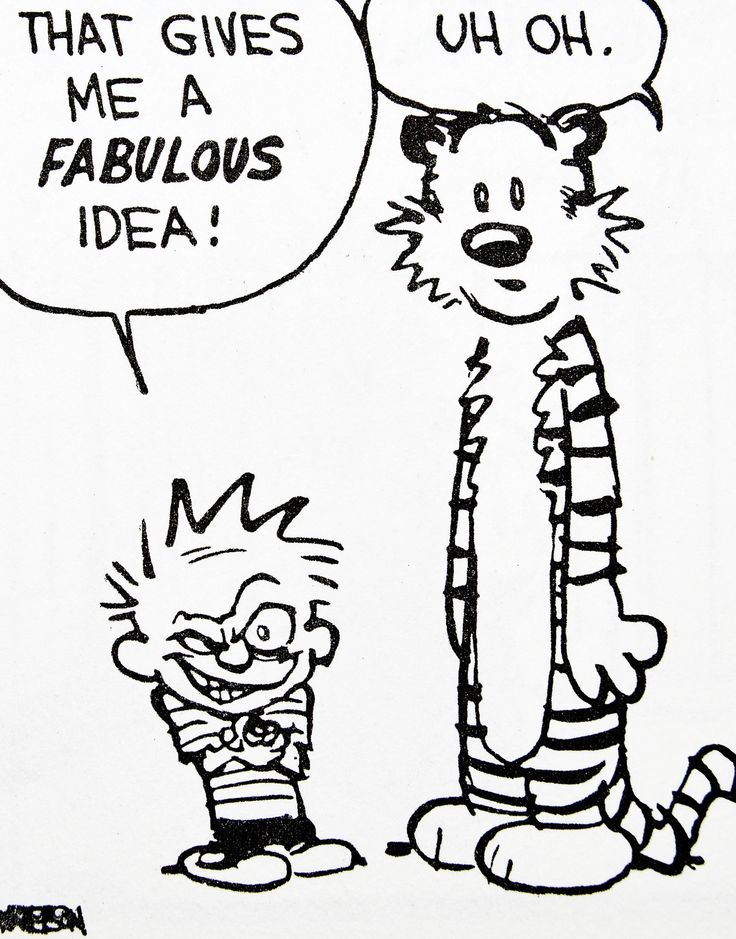
\includegraphics[width=0.6\textwidth]{project_mood_S2}
    \caption*{\textit{Calvin and Hobbes}, Bill Watterson}
\end{figure}

\chapter{Cahier des charges}

Cette fois-ci, pas de changement nécessaire sur la répartition des tâches.

\vspace{1cm}

\begin{center}
    \begin{tabular}{@{} l *4c @{}}
        \toprule
        \multicolumn{1}{c}{}    & \textbf{Soutenance 1}  & \textbf{Soutenance 2}  & \textbf{Soutenance 3} \\ 
        \midrule
        Map & 65\% & 100\% & 100\% \\
        IA & 30\% & 70\% & 100\% \\
        Réseau & 30\% & 75\% & 100\% \\
        Assets & 50\% & 100\% & 100\% \\
        Interface & 10\% & 80\% & 100\% \\
        Site & 10\% & 95\% & 100\% \\
        Gameplay & 40\% & 80\% & 100\% \\
        Budget pizza & 100\% & 60\% & null\\
        \midrule
        Jouabilité & 25\% & 60\% & 100\% \\
        \bottomrule
    \end{tabular}
\end{center}

\vspace{0.5cm}

Les assets étant finalement terminés, l’interface - actuellement en retard,
plutôt 70\% que 80\% - pourra avancer rapidement et être terminée sous peu.

Le site web n’a pas réellement eu besoin d’être amélioré depuis la première
soutenance, mis à part une mise à jour des informations.

Toutes les fonctionnalités de la map sont désormais en place, il restera
toujours quelques légers peaufinements pour la soutenance finale.

L’IA a progressé comme prévue, son fonctionnement sera détaillé plus bas.

Le gameplay a également atteint ses objectifs, les unités sont implémentées et
fonctionnelles, les villes sont utilisables, le Player fait partie intégrante
du jeu, il ne reste maintenant qu’à implémenter une économie au jeu grâce aux
ressources et aux bâtiments des villes ; et à prendre les biomes en compte dans
les calculs des unités.

\chapter{Avancement}

\section{Map (Thibault)}

La première chose qu'il a fallu intégrer à la map était les unités en elles
mêmes. Le système de pathfinding était déjà en place, mais le fait de
positionner les unités, de pouvoir les sélectionner, les déplacer, représentait
une tâche importante et majeure du jeu. 

En utilisant des courbes de Bézier nous avons désormais des déplacements fluides
et assez naturels sur la carte, d'autant plus que ces courbes nous permettent de
gérer facilement l'orientation des unités qui se tournent avant et pendant leurs
déplacements.

Lors de la soutenance précédente nous avions mis en place des menus pour éditer
la carte afin de montrer les différentes fonctionnalités. Nous avons décidé de
réutiliser cette partie pour mettre en place un éditeur de map afin de créer ses
propres cartes sur lesquelles on pourra ensuite jouer.

\begin{figure}[H]
    \centering
    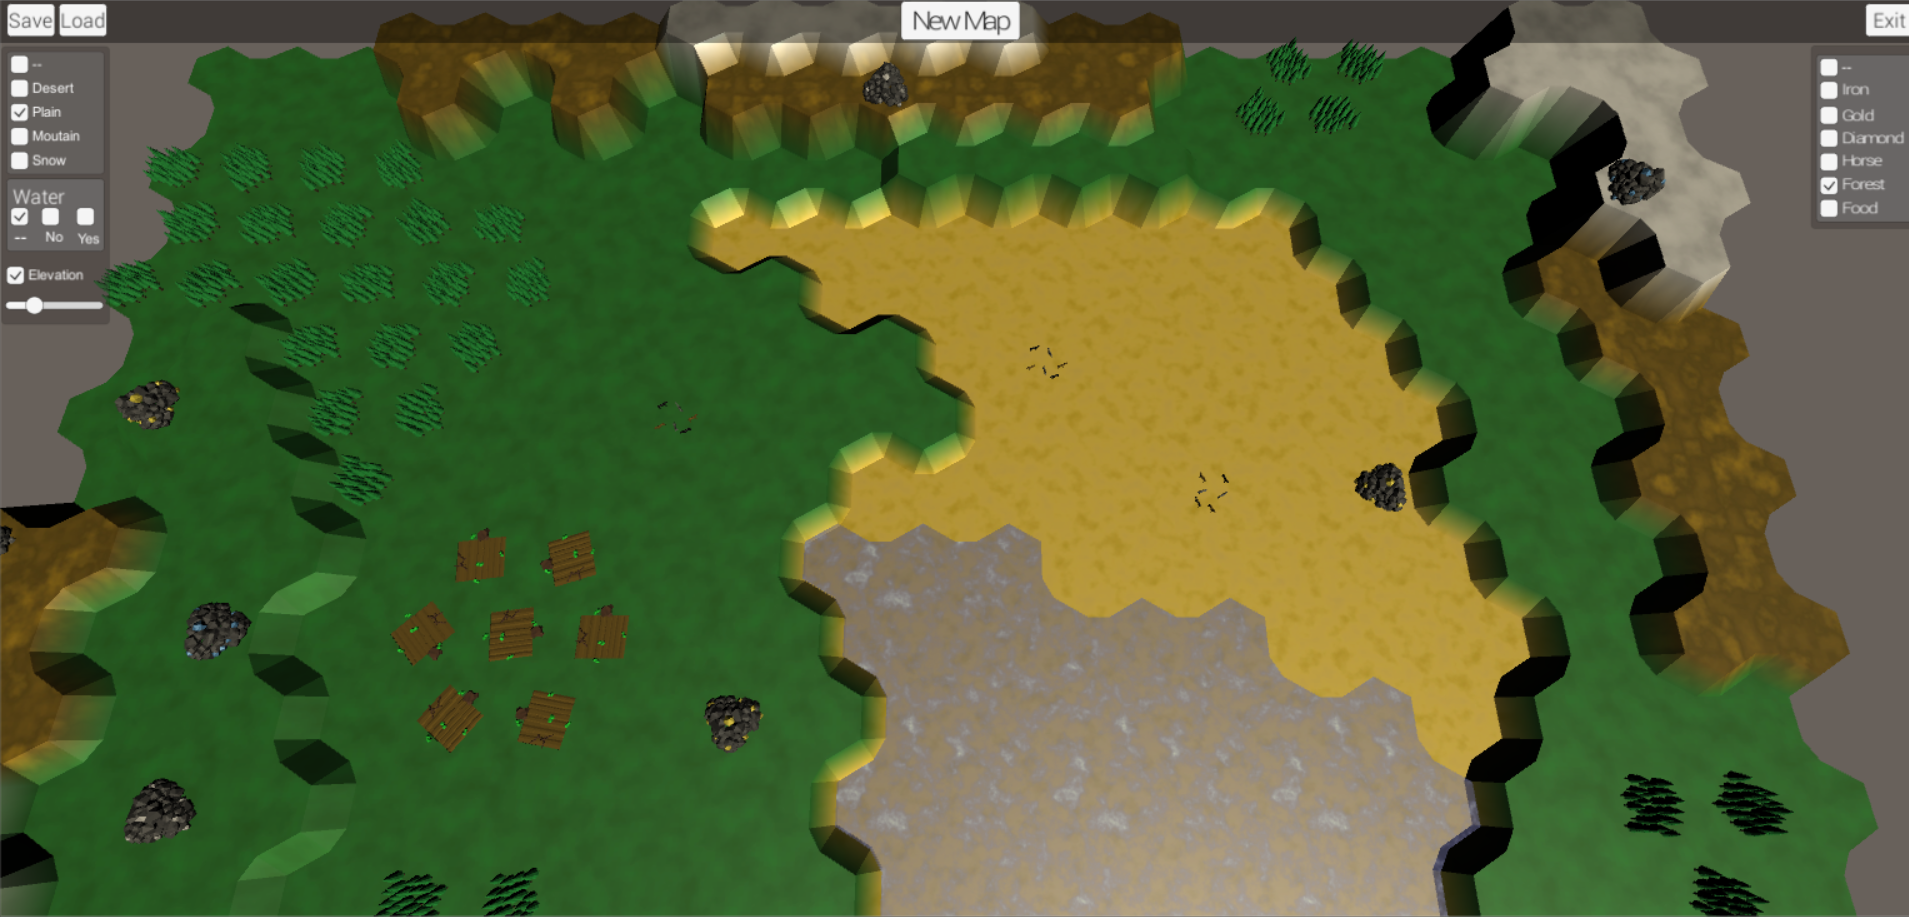
\includegraphics[width=0.8\textwidth]{EditorScreen}
    \caption{Editeur de map}
\end{figure}

Cependant, il était prévu depuis le début de générer des cartes lors d'un début
de partie pour avoir à chaque nouveau lancement de jeu une situation différente.

Une génération de carte procédurale est désormais intégrée au jeu, et le joueur
peut maintenant sélectionner s'il souhaite utiliser une carte qu'il a lui même
édité ou bien en générer une nouvelle.

\begin{figure}[H]
    \centering
    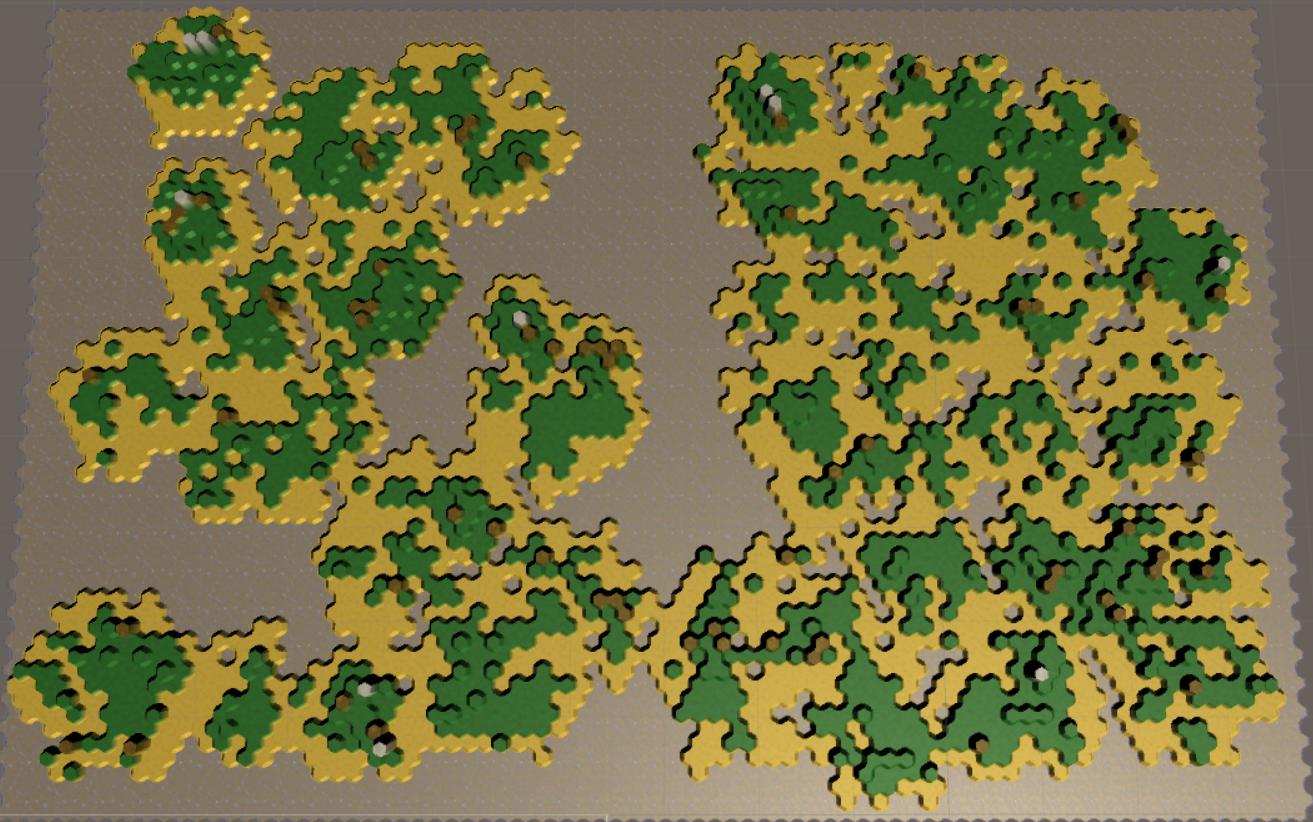
\includegraphics[width=0.8\textwidth]{MapGen1}
    \caption{Génération de carte 1}
\end{figure}

\begin{figure}[H]
    \centering
    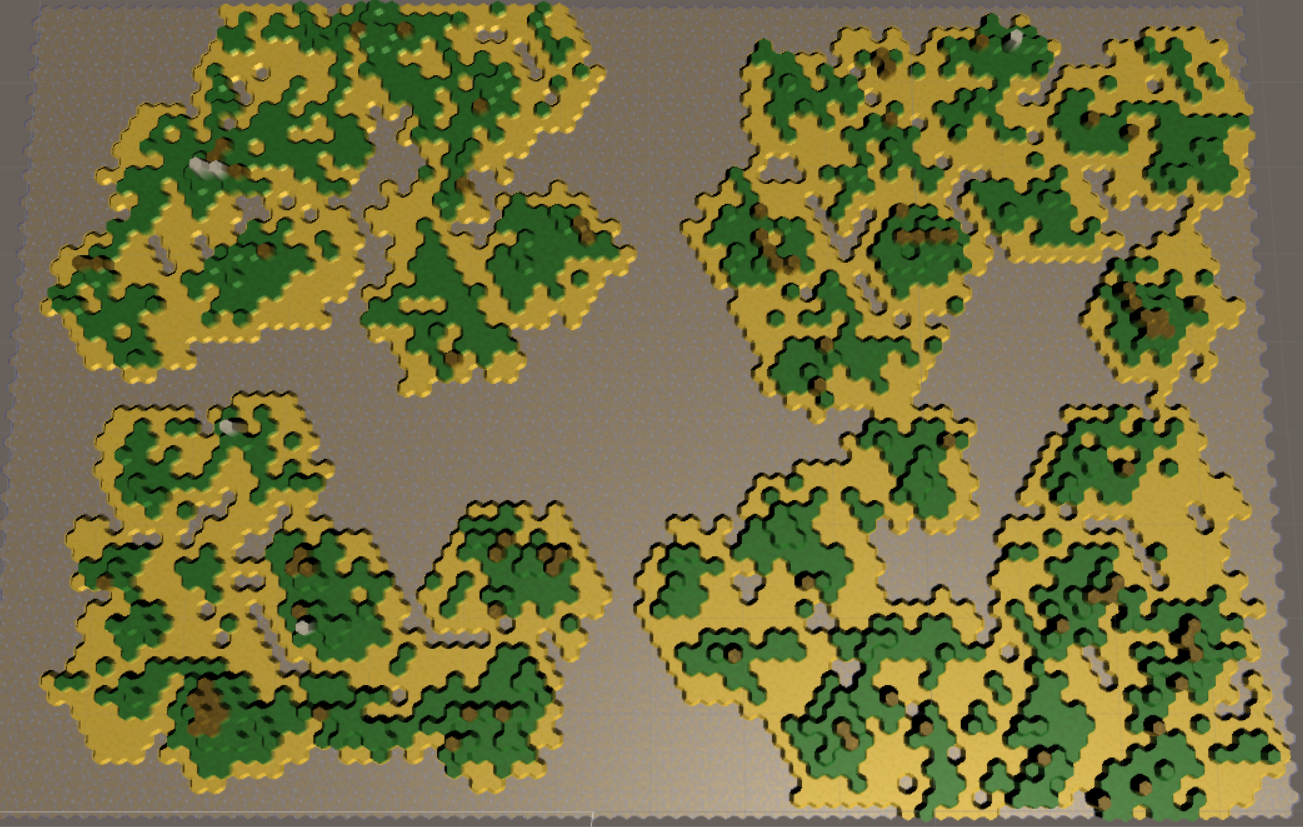
\includegraphics[width=0.8\textwidth]{MapGen2}
    \caption{Génération de carte 2}
\end{figure}

La dernière fonctionnalité que nous voulions intégrer à la carte de Pacification
était le brouillard de guerre, élément indispensable pour ce type de jeu de
stratégie. Il a fallu adapter les shaders ainsi que les textures pour cacher ou
montrer des parties de la carte en fonction de plusieurs critères comme : la
hauteur de la case sur laquelle se trouve l'unité, son nombre de point de
vision, si la case a déjà été visité ou non. On différencie donc deux types de
brouillard : d'une part les terrains inexplorés qui sont totalement cachés du
joueur et de l'autre les terrain précédemments explorés mais hors de vision et
portée de l'unité.

\begin{figure}[H]
    \centering
    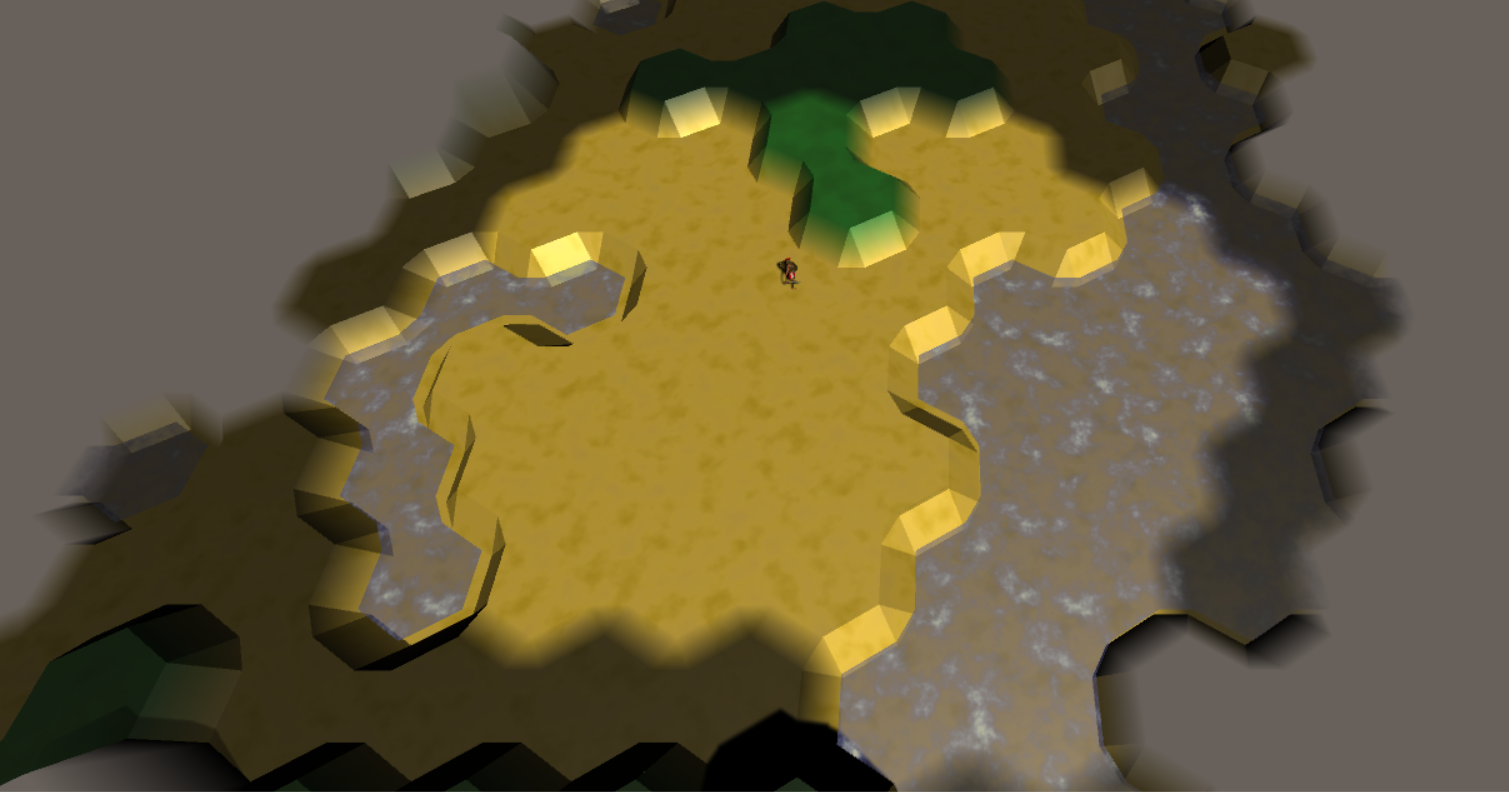
\includegraphics[width=0.8\textwidth]{FogOfWar}
    \caption{Brouillard de guerre}
\end{figure}

\section{Réseau et multijoueur (Valérian)}

\section{Gameplay (Antoine)}

Le gameplay a bien avancé. Nous disposons à présent d’unités correctement
implémentées.

Au début de la partie, le joueur commence avec un colon et un fantassin. Le
colon permet de construire la première ville du joueur, tandis que l’unité
offensive peut permettre d’explorer les alentours et de découvrir la carte,
alors recouverte par le brouillard de guerre. 

\begin{figure}[H]
    \centering
    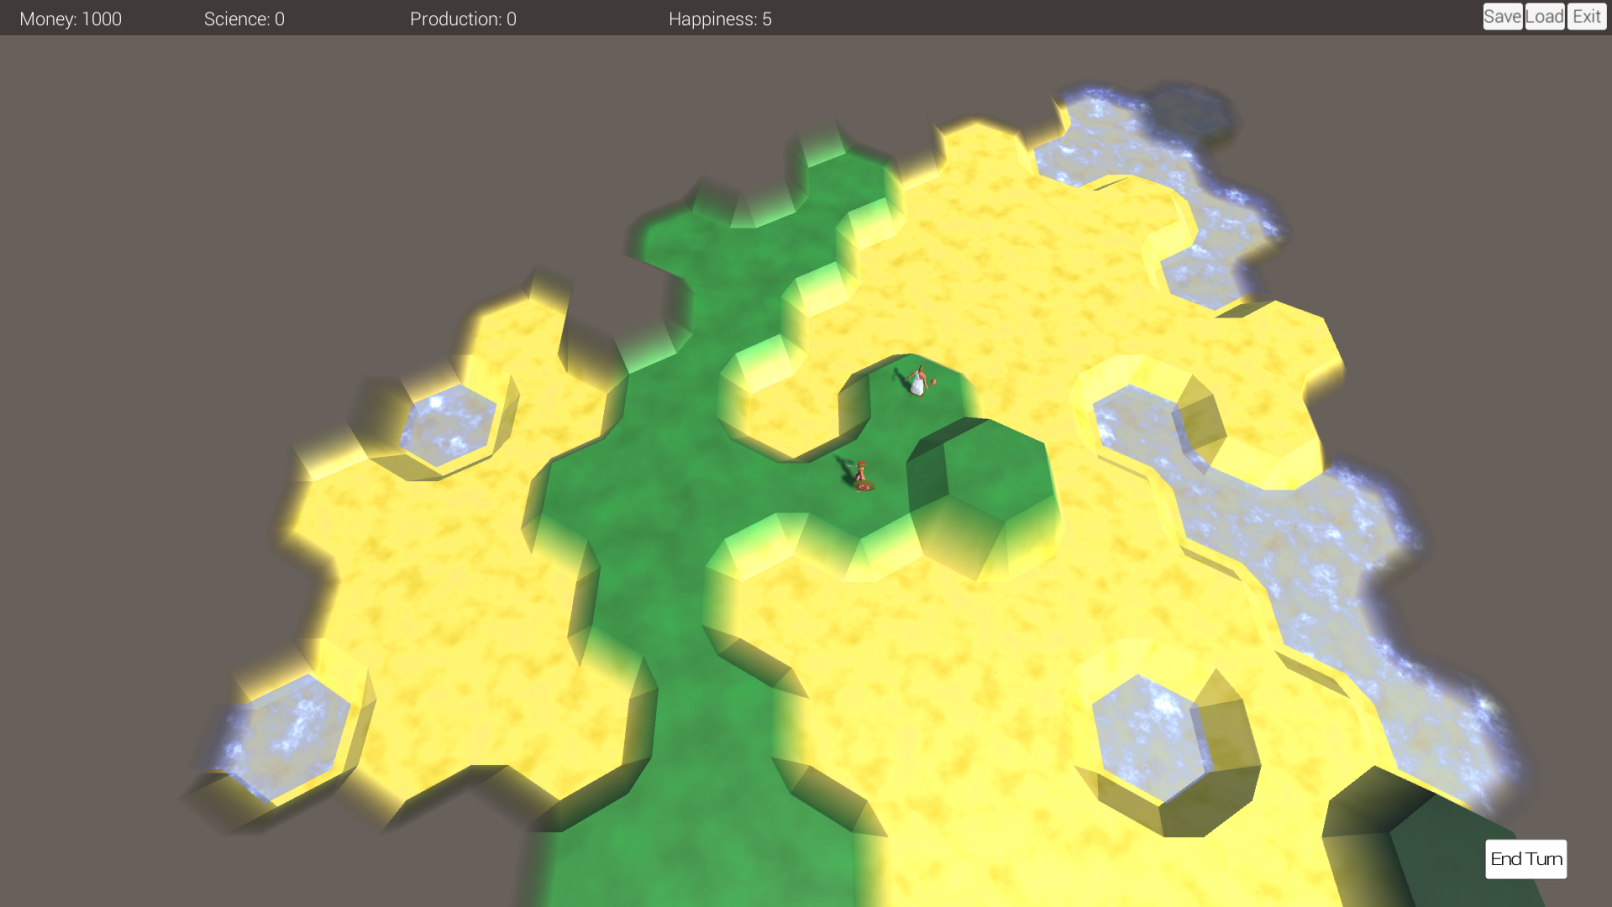
\includegraphics[width=0.8\textwidth]{InitialSituation}
    \caption{Situation initiale}
\end{figure}

Les unités peuvent donc se déplacer et activer leur action propre (construire
une ville pour le colon, exploiter une ressource pour l'ouvrier, attaquer un 
ennemie pour les unités offensives).

\begin{figure}[H]
    \centering
    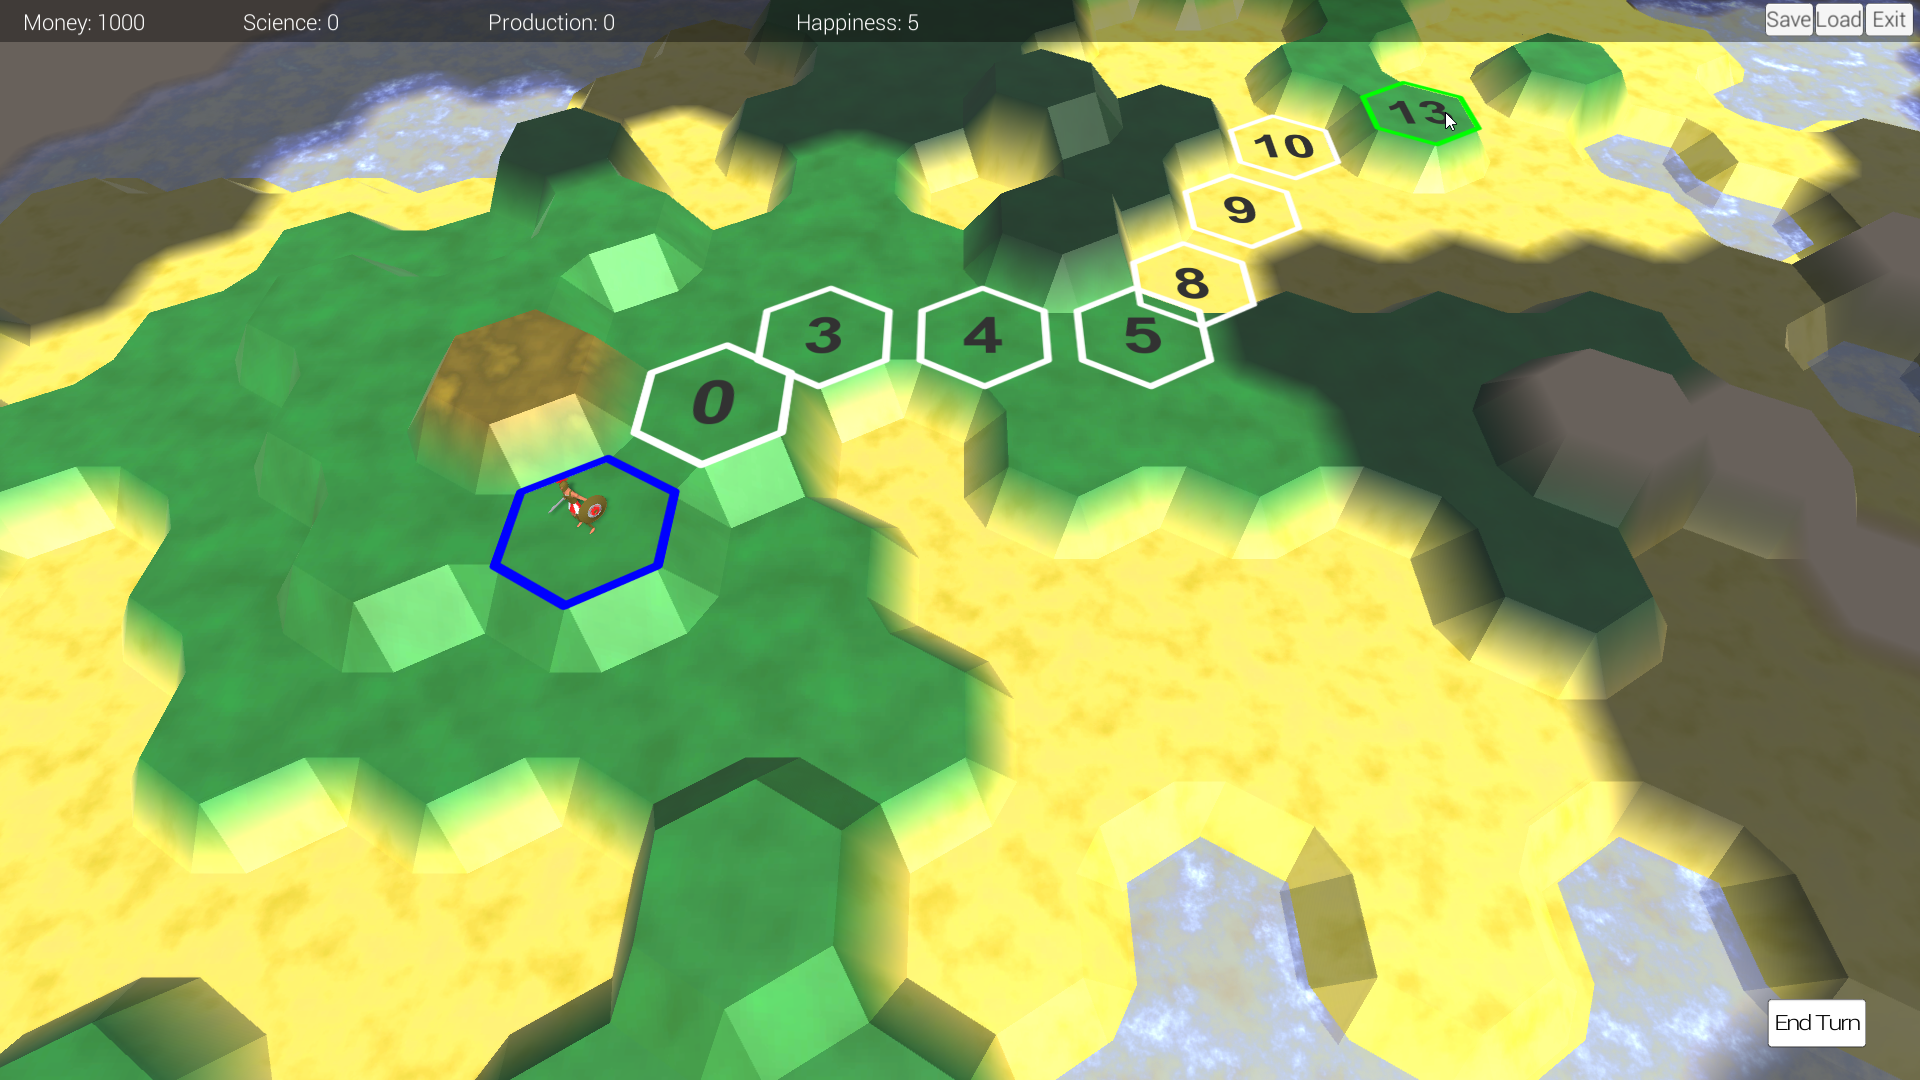
\includegraphics[width=0.8\textwidth]{Pathfinding}
    \caption{Pathfinding}
\end{figure}

La ville permet pour le moment de produire d’autres unités qui apparaîtront dans
dans cette dernière grâce au menu “barrack”. Il est ainsi possible de créer un
autre colon, un travailleur, ou une des différentes unités offensives.

Chaque unité possède des caractéristiques qui lui sont propres, ainsi qu’un
modèle 3D assigné à sa création selon son type (les unités d’attaque possèdent
un second modèle amélioré qu’elles obtiennent à partir du niveau 11). Ces
statistiques, présentées dans les tableaux de la première soutenance, influeront
notamment sur le nombre de tour nécessaire pour tuer une cible et  la vitesse de
déplacement.

La ville disposera également d’améliorations, cependant elles dépendent de la
population ainsi que de l’économie qui seront implémentés lors de la dernière
phase de développement.

\section{Assets (Cédric)}

Les assets ont été finis à 100\%, les modèles 3D sont basés, pour la plupart,
sur mes premières créations pour faire les suivantes. Trois nouvelles textures
ont été créées spécialement pour les villes.

\begin{figure}[H]
    \centering
    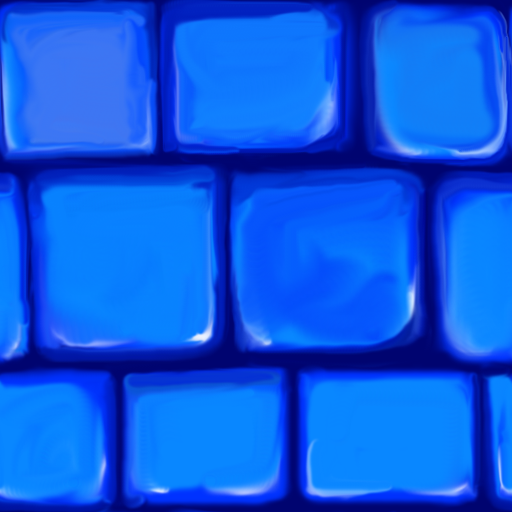
\includegraphics[width=0.3\textwidth]{BlueRoof}
    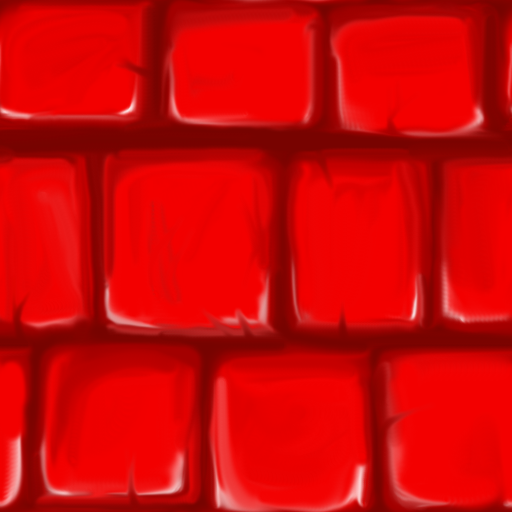
\includegraphics[width=0.3\textwidth]{RedRoof}
    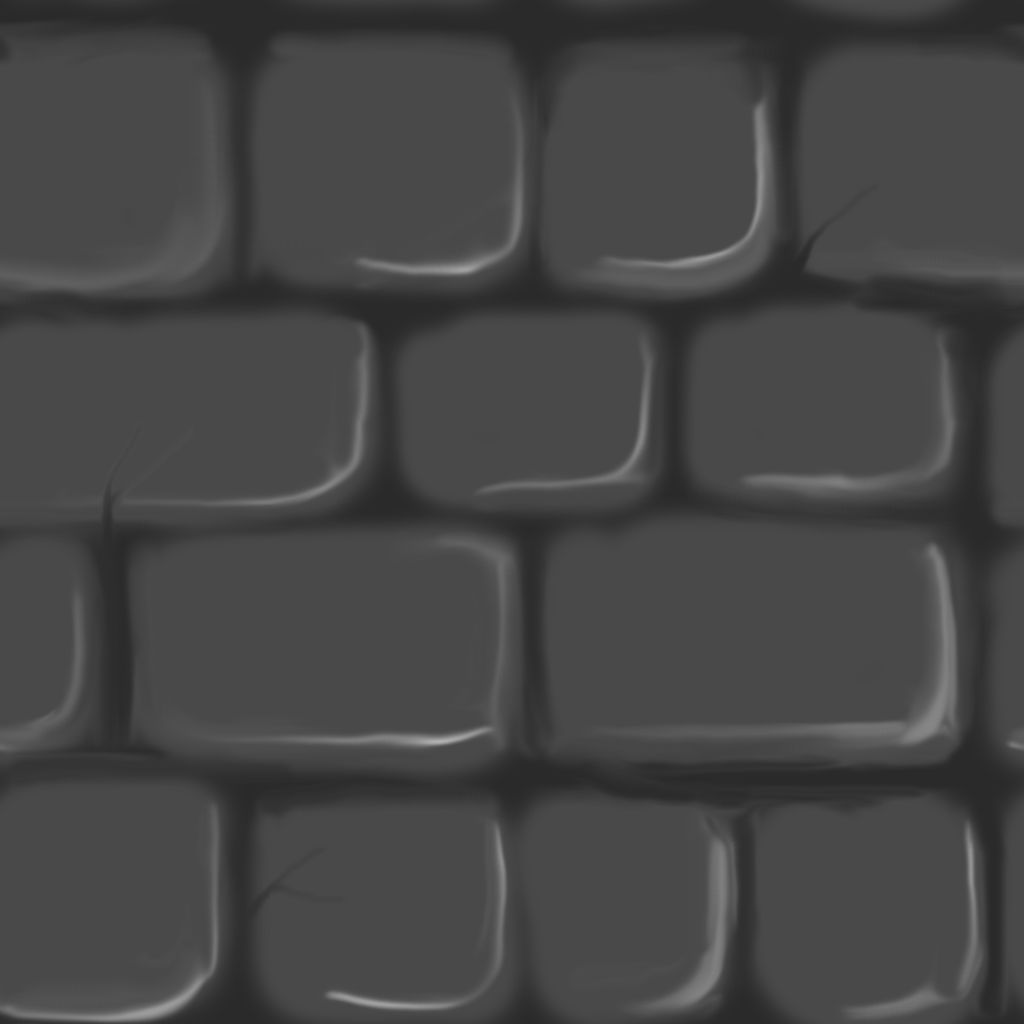
\includegraphics[width=0.3\textwidth]{DarkStoneWall}
    \caption{BlueRoof, RedRoof, DarkStoneWall}
\end{figure}

Les modèles 3D des bâtiments sont tous finis. Seuls les villes ont nécessité de
nouveaux modèles car ceux de la dernière soutenance ont pu être réutilisé comme
prévu pour gagner du temps. Il existe deux modèles différents pour les
ressources du jeu : la version naturelle et la version exploitée.

\begin{figure}[H]
    \centering
    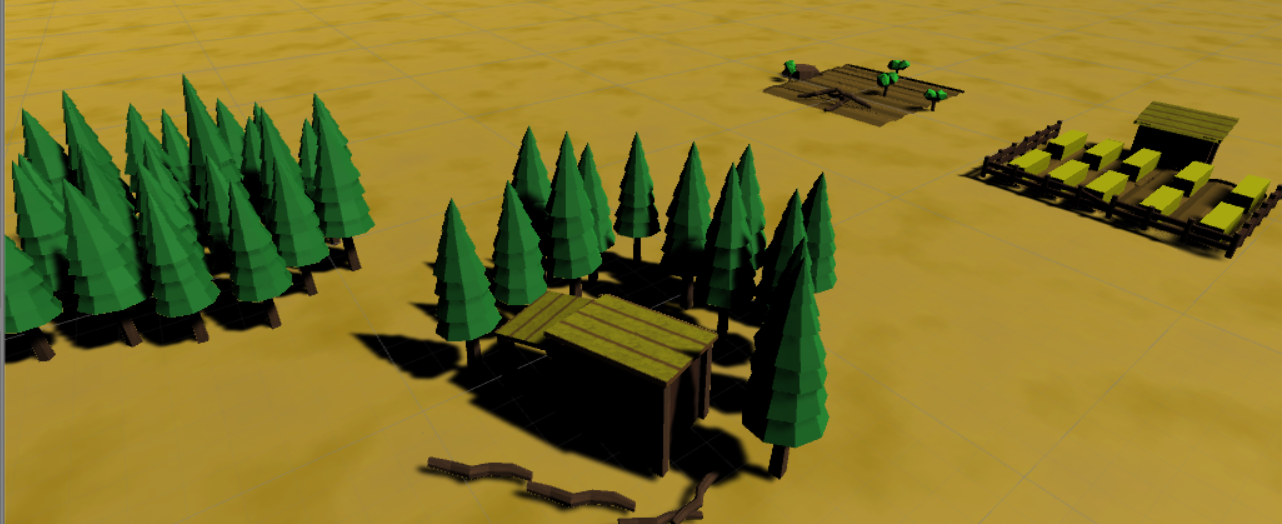
\includegraphics[width=0.8\textwidth]{assets_food_forest}
    \caption{Forêt naturelle et exploitée}
\end{figure}

\begin{figure}[H]
    \centering
    \includegraphics[width=0.8\textwidth]{}
    \caption{Les différents modèles de ville}
\end{figure}

Concernant les unités ajoutées il y a les deux versions d’unité à portée, les
deux versions des unités de siège (catapulte et canon), et le cavalier qui
correspond à l’amélioration de l’infanterie. Comme pour les modèles précédent,
la création des unités (notamment le canon et la catapulte) se sont fait à
l’aide d’image de référence. Les modèles des unités humaines ont été construits
à partir du modèle humain de base créer durant la première période du projet.

\begin{figure}[H]
    \centering
    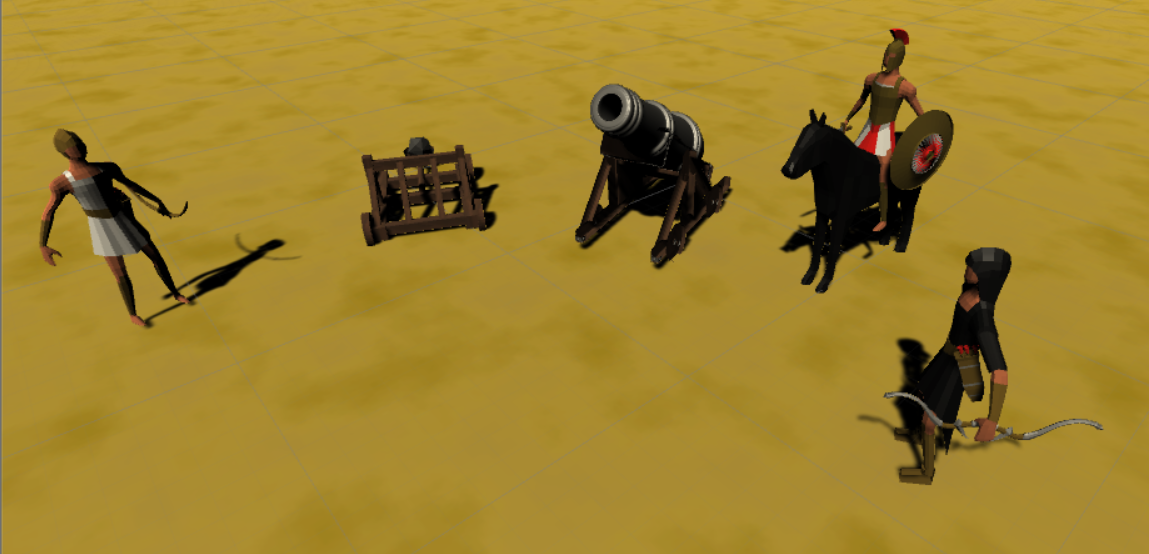
\includegraphics[width=0.8\textwidth]{NewUnitsScreen}
    \caption{Nouvelles unités}
\end{figure}

Les animations des personnages ont toujours été considéré comme du bonus.
Cependant, des premiers tests pour la catapulte ont été faits, mais ne sont pas
encore intégrés au jeu. Ces animations pourront être réutilisées par la suite
par le canon ou d'autres unités. L'animation des armatures humaines semblent
assez complexe à gérer, d'où l'utilisation d'un outil externe hébergé par le
site internet gratuit mixamo.com permettant de donner simplement une armature à
un personnage avec des animations fluides.

\section{Interface (Cédric, Valérian, Antoine)}

Pour le menu nous avons récupéré un menu créé par MICHSKY qui l’a rendu
accessible à tous gratuitement sur internet. Nous l’avons aménagé de manière à
ce qu’il s’adapte parfaitement à notre jeu.

\begin{figure}[H]
    \centering
    \includegraphics[width=0.8\textwidth]{}
    \caption{MainMenu}
\end{figure}

Le menu principal comporte un accès au “menu Play” qui regroupe les
fonctionnalités du jeu en solo et du jeu en multijoueur.

\begin{figure}[H]
    \centering
    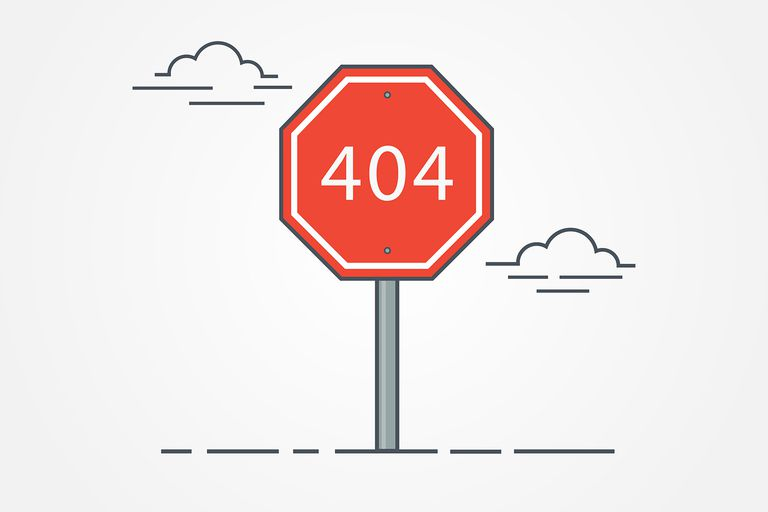
\includegraphics[width=0.8\textwidth]{404}
    \caption{MenuPlay}
\end{figure}

Les images apparaissant sur les boutons “Solo” “Host” et “Join” ont été faites
grâce à blender. Les positions du soldat ont été possible grâce à l’armature
et aux animations importés sur le site Mixamo.com cité prècedemment. Un menu
“Paramètres” a été créé où l’on pourra par exemple changer la langue du jeu ou
activer/désactiver du jeu. Un bouton “information”s est disponible et mène aux
crédits du jeu.  On navigue de menu en menu grâce à des déplacements de
caméras qui nous amènent sur des nouveaux canvas et des boutons back ont été
placé pour simplifier cette navigation.

%Le logo pacification a été créé sur le site FontStruct.com en s’inspirant d’un modèle trouvé sur internet. Pour insérer le titre correctement importer la police d’écriture ne suffisait pas car le texte apparaissait flou. Nous avons donc mis une image du texte. Pour cela nous avons utilisé le logiciel open source Krita qui a permis d’écrire et de rendre le fond transparent afin que le mot “Pacification” apparaisse sans fond sur le menu.

De la musique a été ajoutée dans le jeu.

L’interface de la caserne (barrack) est reliée aux villes. Sa position et son
échelle actuelle seront peut-être amenée à changer, l’interface actuelle
n’étant pas encore parfaitement organisée. 

\section{IA (Thibault)}

\section{Site Web (Valérian)}

\chapter{Avances, retards, difficultés rencontrées}

\section*{Map}

\section*{Réseau et Multijoueur}

\section*{Gameplay}

Si on reprend la hiérarchie des classes présentée lors de la première
soutenance, on peut voir que les unités sont complètement implémentées, et les
villes le sont en partie (l’économie reste à implémenter). Le “Player” est
également géré par le réseau et permet de coordonner les villes et les unités.
Les biomes sont présents dans le code, mais pour le moment ils ne sont pas pris
en compte par le pathfinding et la génération de la map: il reste à organiser
une probabilité d’apparition des différentes ressources.

\begin{figure}[H]
    \centering
    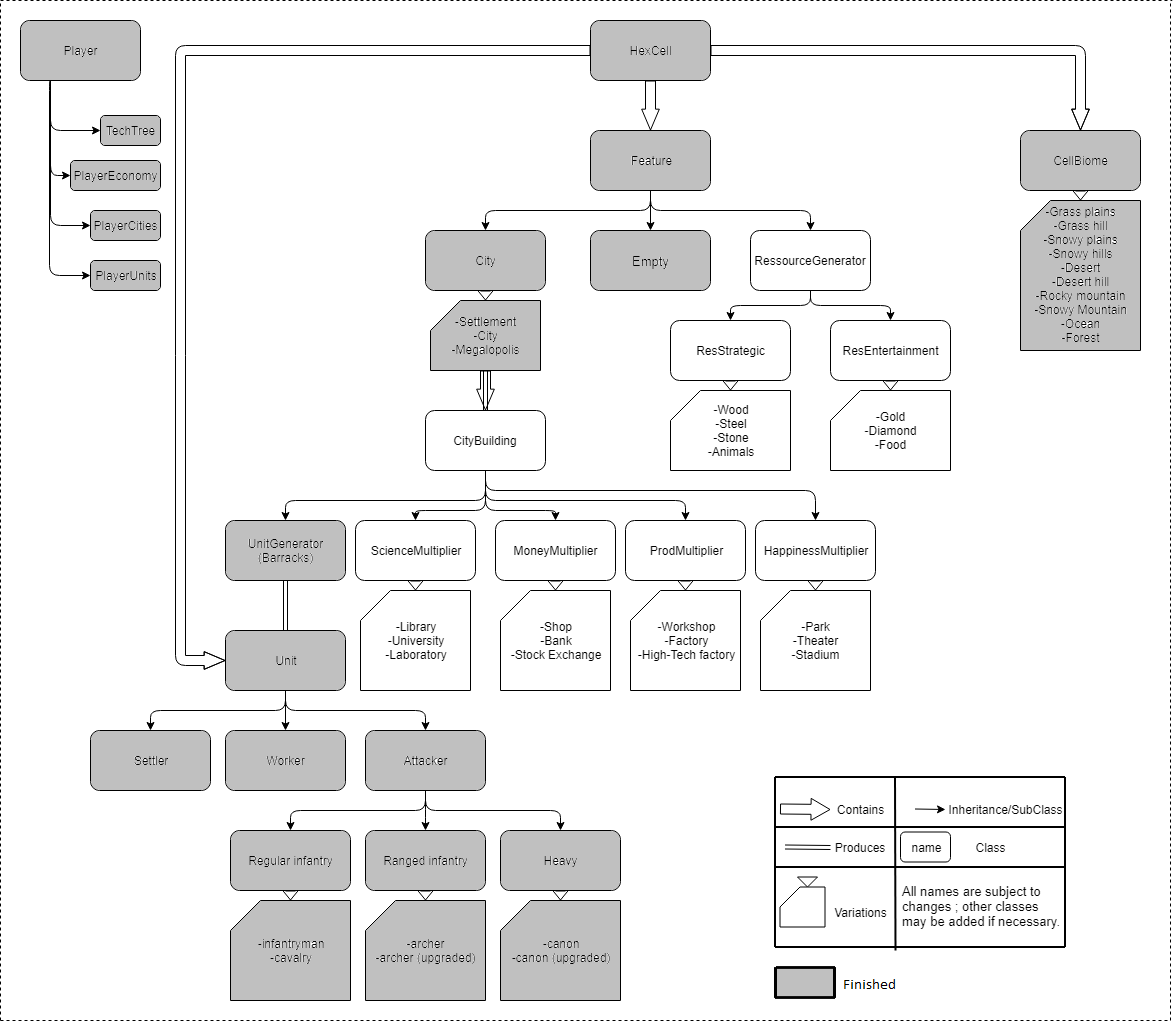
\includegraphics[width=1\textwidth]{class_hierarchy}
    \caption{hiérarchie (avancement)}
\end{figure}

Pour la soutenance finale, il reste donc à implémenter l’économie du jeu (donc
les bâtiments des villes et les ressources) et adapter les paramètres des
biomes/troupes afin d’obtenir un jeu le plus équilibré possible.

La difficulté principale durant cette période a été d'apprendre à "lier" les
classes selon Unity (qui doivent être instanciées pour être affichées sur la
map), et celles de C\# qui appellent un constructeur (dont j'avais besoin pour
gérer les unités et les villes), sans pour autant créer de conflits avec les
autres systèmes eux aussi nécessaires au fonctionnement du jeu. Cela m'a pris
plus de temps que prévu et a été une source de stress, mais tout a fini par
fonctionner.

\section*{Assets}

\section*{Interface}

\section*{IA}

\section*{Site web}

\chapter{À venir}

Pour la troisième et dernière soutenance, nous allons devoir terminer
\textit{Pacification}. Ce qui signifie mettre en place l'économie et équilibrer
le gameplay, finir l'interface pour la rendre la plus confortable et intuitive
possible, ajouter les ressources à la map, terminer l'IA, et bien sûr prendre
le tout en compte dans le réseau qu'il faudra stabiliser.

En somme, beaucoup de travail, mais rien que nous ne puissions faire à temps.
Le jeu ayant déjà bien avancé, et les systèmes principaux étant déjà mis en
place, nous saurons ajouter ces dernières fonctionnalités sans difficulté
majeure.

\chapter{Expériences personnelles}

\begin{itemize}
	\item \textbf{Thibault :} TODO
        \item \textbf{Valérian :} TODO
	\item \textbf{Cédric :} TODO
    \item \textbf{Antoine :} Pour ma part, je suis satisfait de mes avancées,
    bien que, comme expliqué plus haut, je n'avais pas anticipé de telles
    difficultés pour lier les systèmes entre eux et les faire fonctionner
    correctement. Cependant, j'ai pu apprendre de ces problèmes et je sais
    maintenant les résoudre, ce qui me facilitera la tâche lors de la dernière
    phase de développement du projet.
\end{itemize}

\chapter{Conclusion}

\end{document}
